
\chapter{BRI\textsubscript{2} Analysis}\label{ch:Ch.3}

This chapter will explain the $BRI_2$ formula and what are the variables involved in the calculation of the risk index. After that the analysis is reported to understand its behavior, the possible limitations and the correlation between the index and the wildlife strike events.
In particular the focus will be on the sensitivity of sightings and $BRI_2$ correlation estimation.

\section{Formula explanation}\label{Formula_explanation}
In order to determine the $BRI_2$, 17 functional groups have been identified, Table \ref{tab-bird_species} , composed of species not strictly taxonomically linked but with common ecological, behavioural and physical characteristics \cite{ENACcircolareAPT_01B}.
\\
The following factors are calculated for each functional group:

\begin{itemize}
    \item $\overline{W}$: the average weight of the $i^{th}$ functional group since monitoring the activity started.
    \item $Ag$: the group specific aggregation index, average number of flocks sighted at the airport since monitoring the activity started.
    \item $BS$: the number of impacts recorded for the $i^{th}$ functional group.
    \item $TFN$: the mean value of flights per year.
    \item $\overline{TFN}$: the mean value of flights per month.
    \item $EOF^{95}$: the 95th percentile of the EOF (Effect On Flight, Table \ref{tab-EOF}).
    \item $DB$: the mean daily number of birds of the $i^{th}$ functional group.
    \item $DF$: the mean daily flight traffic calculated on a monthly basis.
\end{itemize}
After calculating these factors it is possible to determine the value of $BRI_2$ using the following 3 equations:

\begin{equation} \label{eq:3.1}
GF_i=\overline{W_i}\cdot Ag_i \cdot\frac{BS_i}{TFN} \cdot EOF_i ^{95} 
\end{equation}

\begin{equation} \label{eq:3.2}
GSR_i=\frac{GF_i}{\sum_{i=1}^{N}GF_i}\cdot DB_i
\end{equation}

\begin{equation} \label{eq:3.3}
BRI_2=\left(\frac{\sum_{i=1}^{N}GSR_i \cdot DF}{\overline{TFN}}\right)
\end{equation}
where $GF_i$ represents the Group Factor and $GSR_i$ the Group Specific Risk. In equations \ref{eq:3.1}, \ref{eq:3.2}, \ref{eq:3.3}, $i$ indicates a species group (Table \ref{tab-bird_species}) and N is the total number of groups.
In order to understand the behaviour of $BRI_2$, an analysis of these parameters was required.

\section{Parameters analysis}\label{parameters_analysis}
Before proceeding with the analysis of the parameters, a precondition is necessary. After researching Italian airports, the airport chosen to show this analysis was Pisa as it is among the best airports for the quality of the data collected.

The first parameter analyzed was $\overline{W}$, which identifies the average weight of the $i^{th}$ group, independently of the number of sightings.
It is possible to observe from the graph in Figure \ref{W_fig} that this parameter is a constant for each species group, so it makes a constant contribution to the calculation of the Group Factor $GF_i$, eq. \ref{eq:3.1}.

\begin{figure}
	\centering
	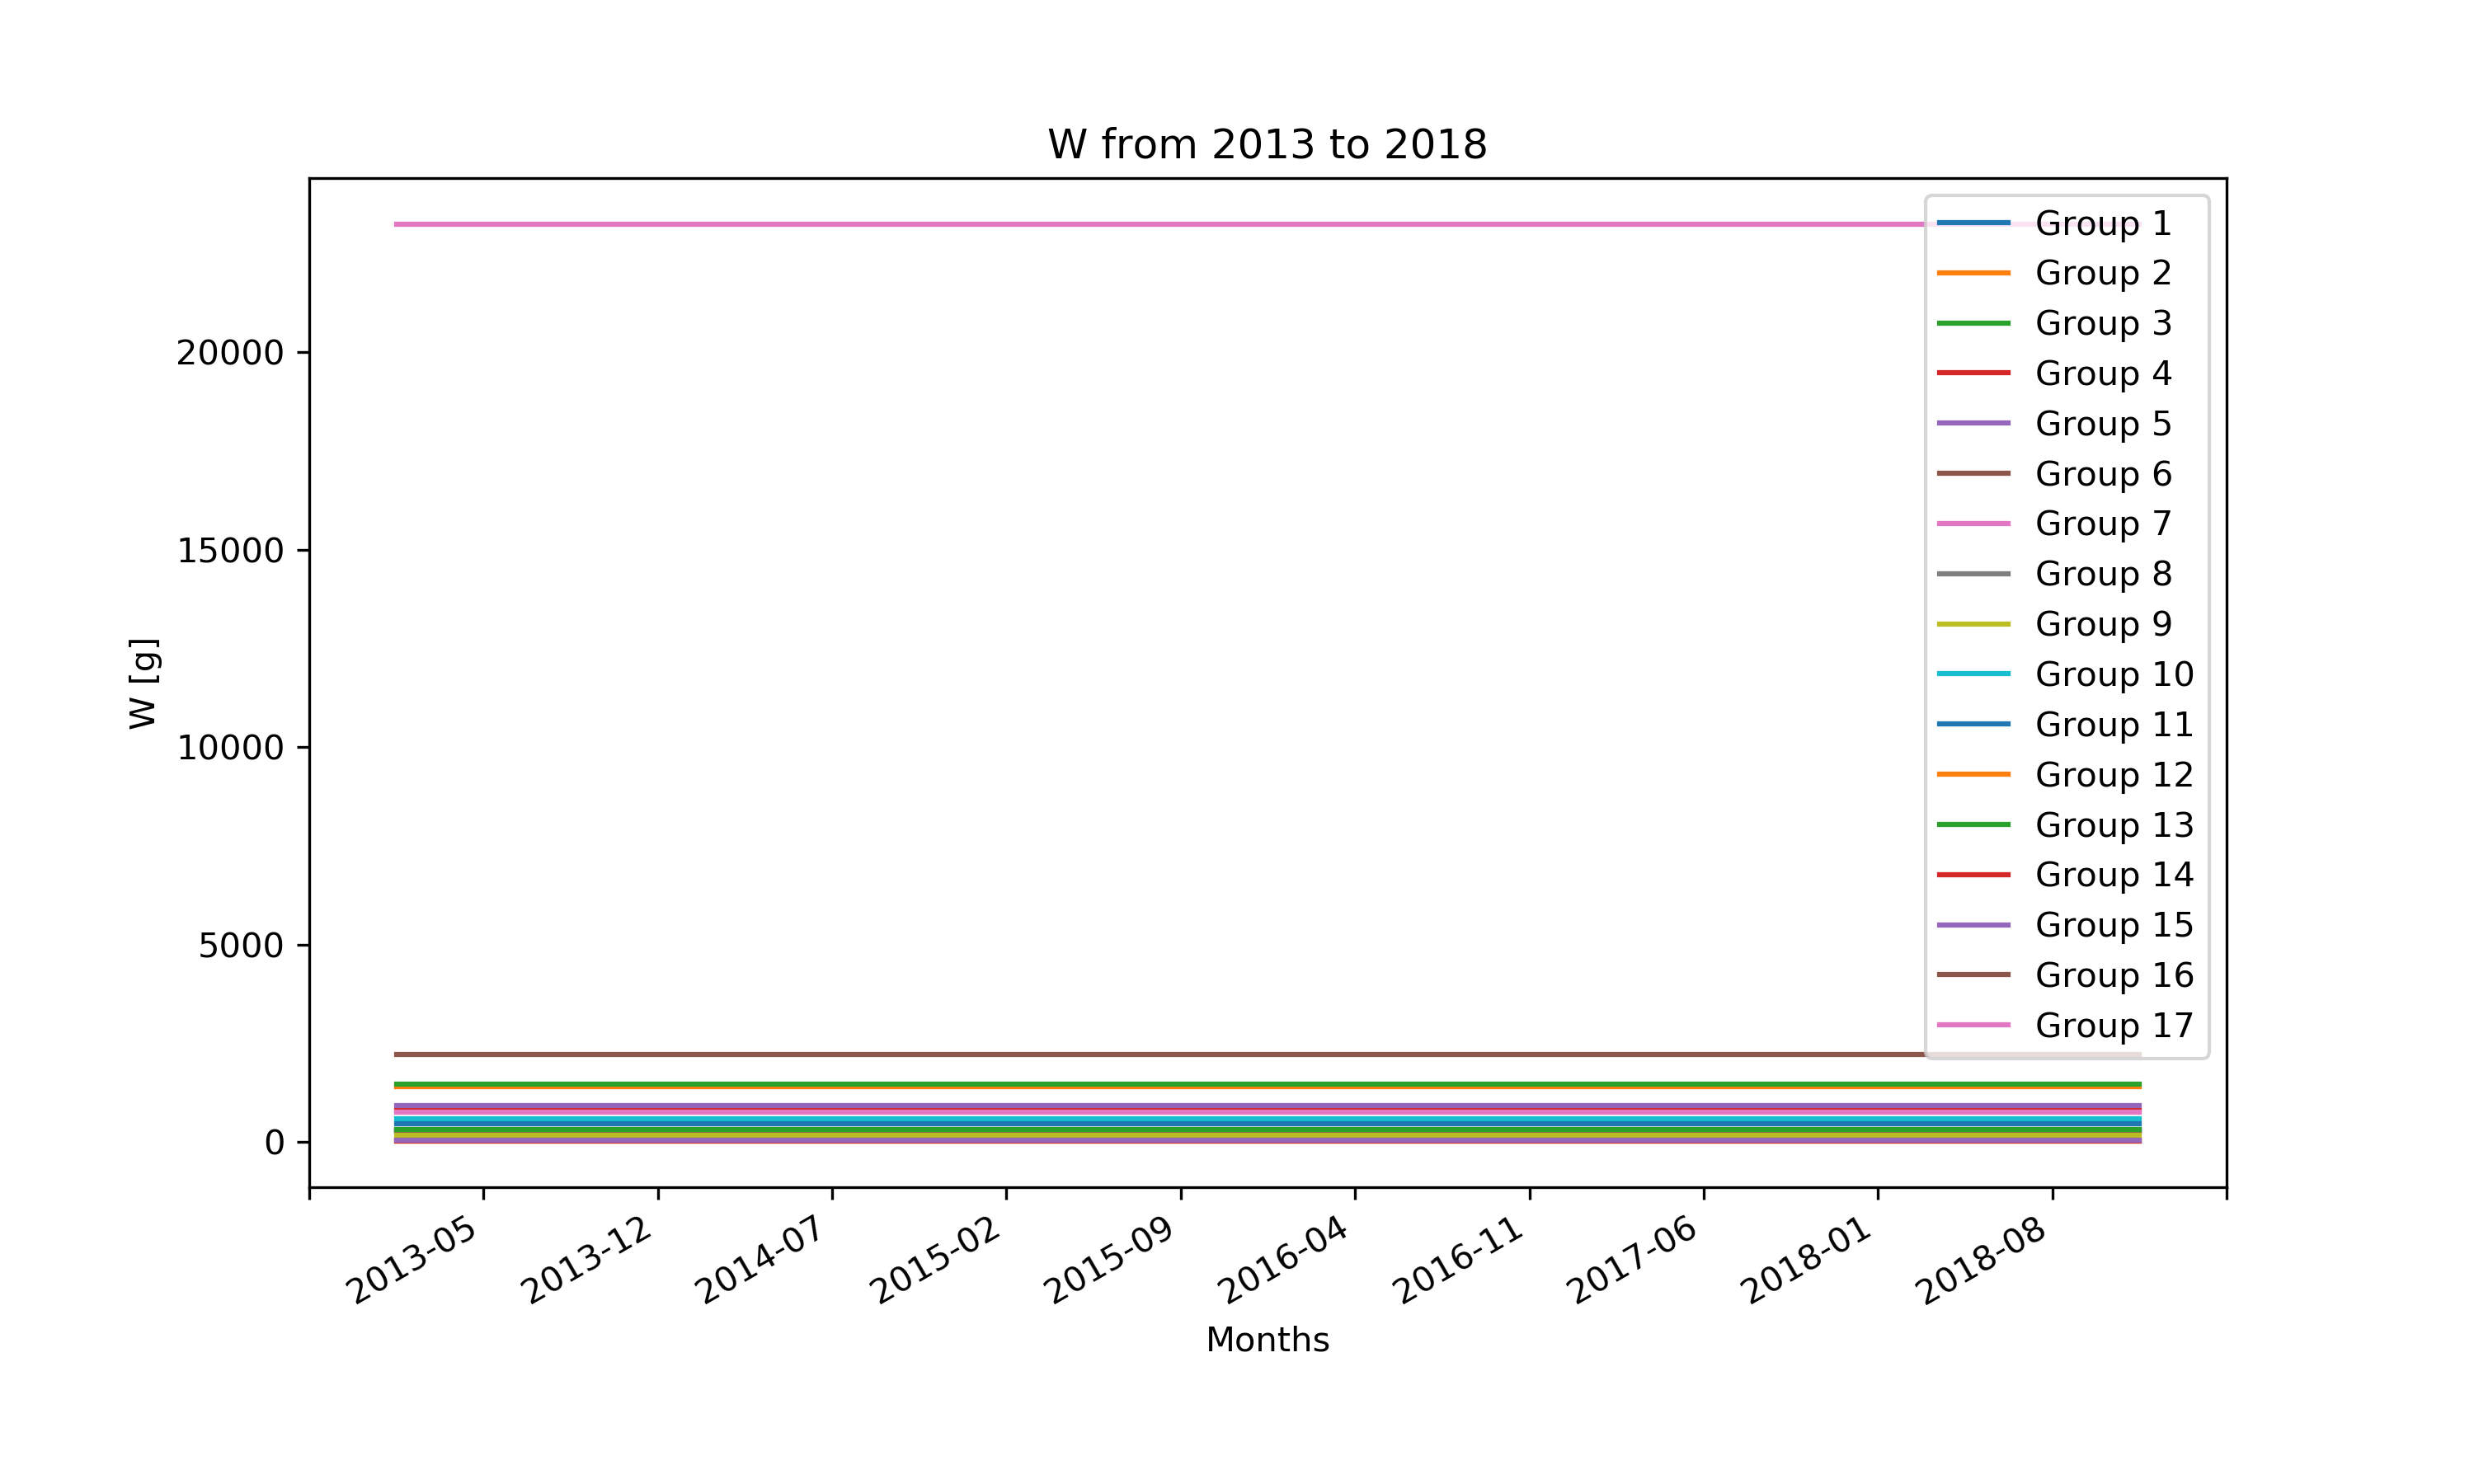
\includegraphics[width=13cm]{img/W.png}
	\caption{$\overline{W}$ parameter from 2013 to 2018 for Pisa airport. The figure shows how over the years analyzed, the weight has remained constant.}
	\label{W_fig}
\end{figure}

The next parameter analysed was $BS$ that is the number of impacts recorded for the $i^{th}$ functional group. This parameter plays an important role in the calculation of the Group Factor. It can only increase (either unchanged) its value as the months increase, as it is not averaged on the calculation period. In the Figure \ref{BS_fig} it is possible see how the BS value is only increased (either unchanged) for each functional group from the beginning of the calculation, 2013, until 2019 excluded.

\begin{figure}
	\centering
	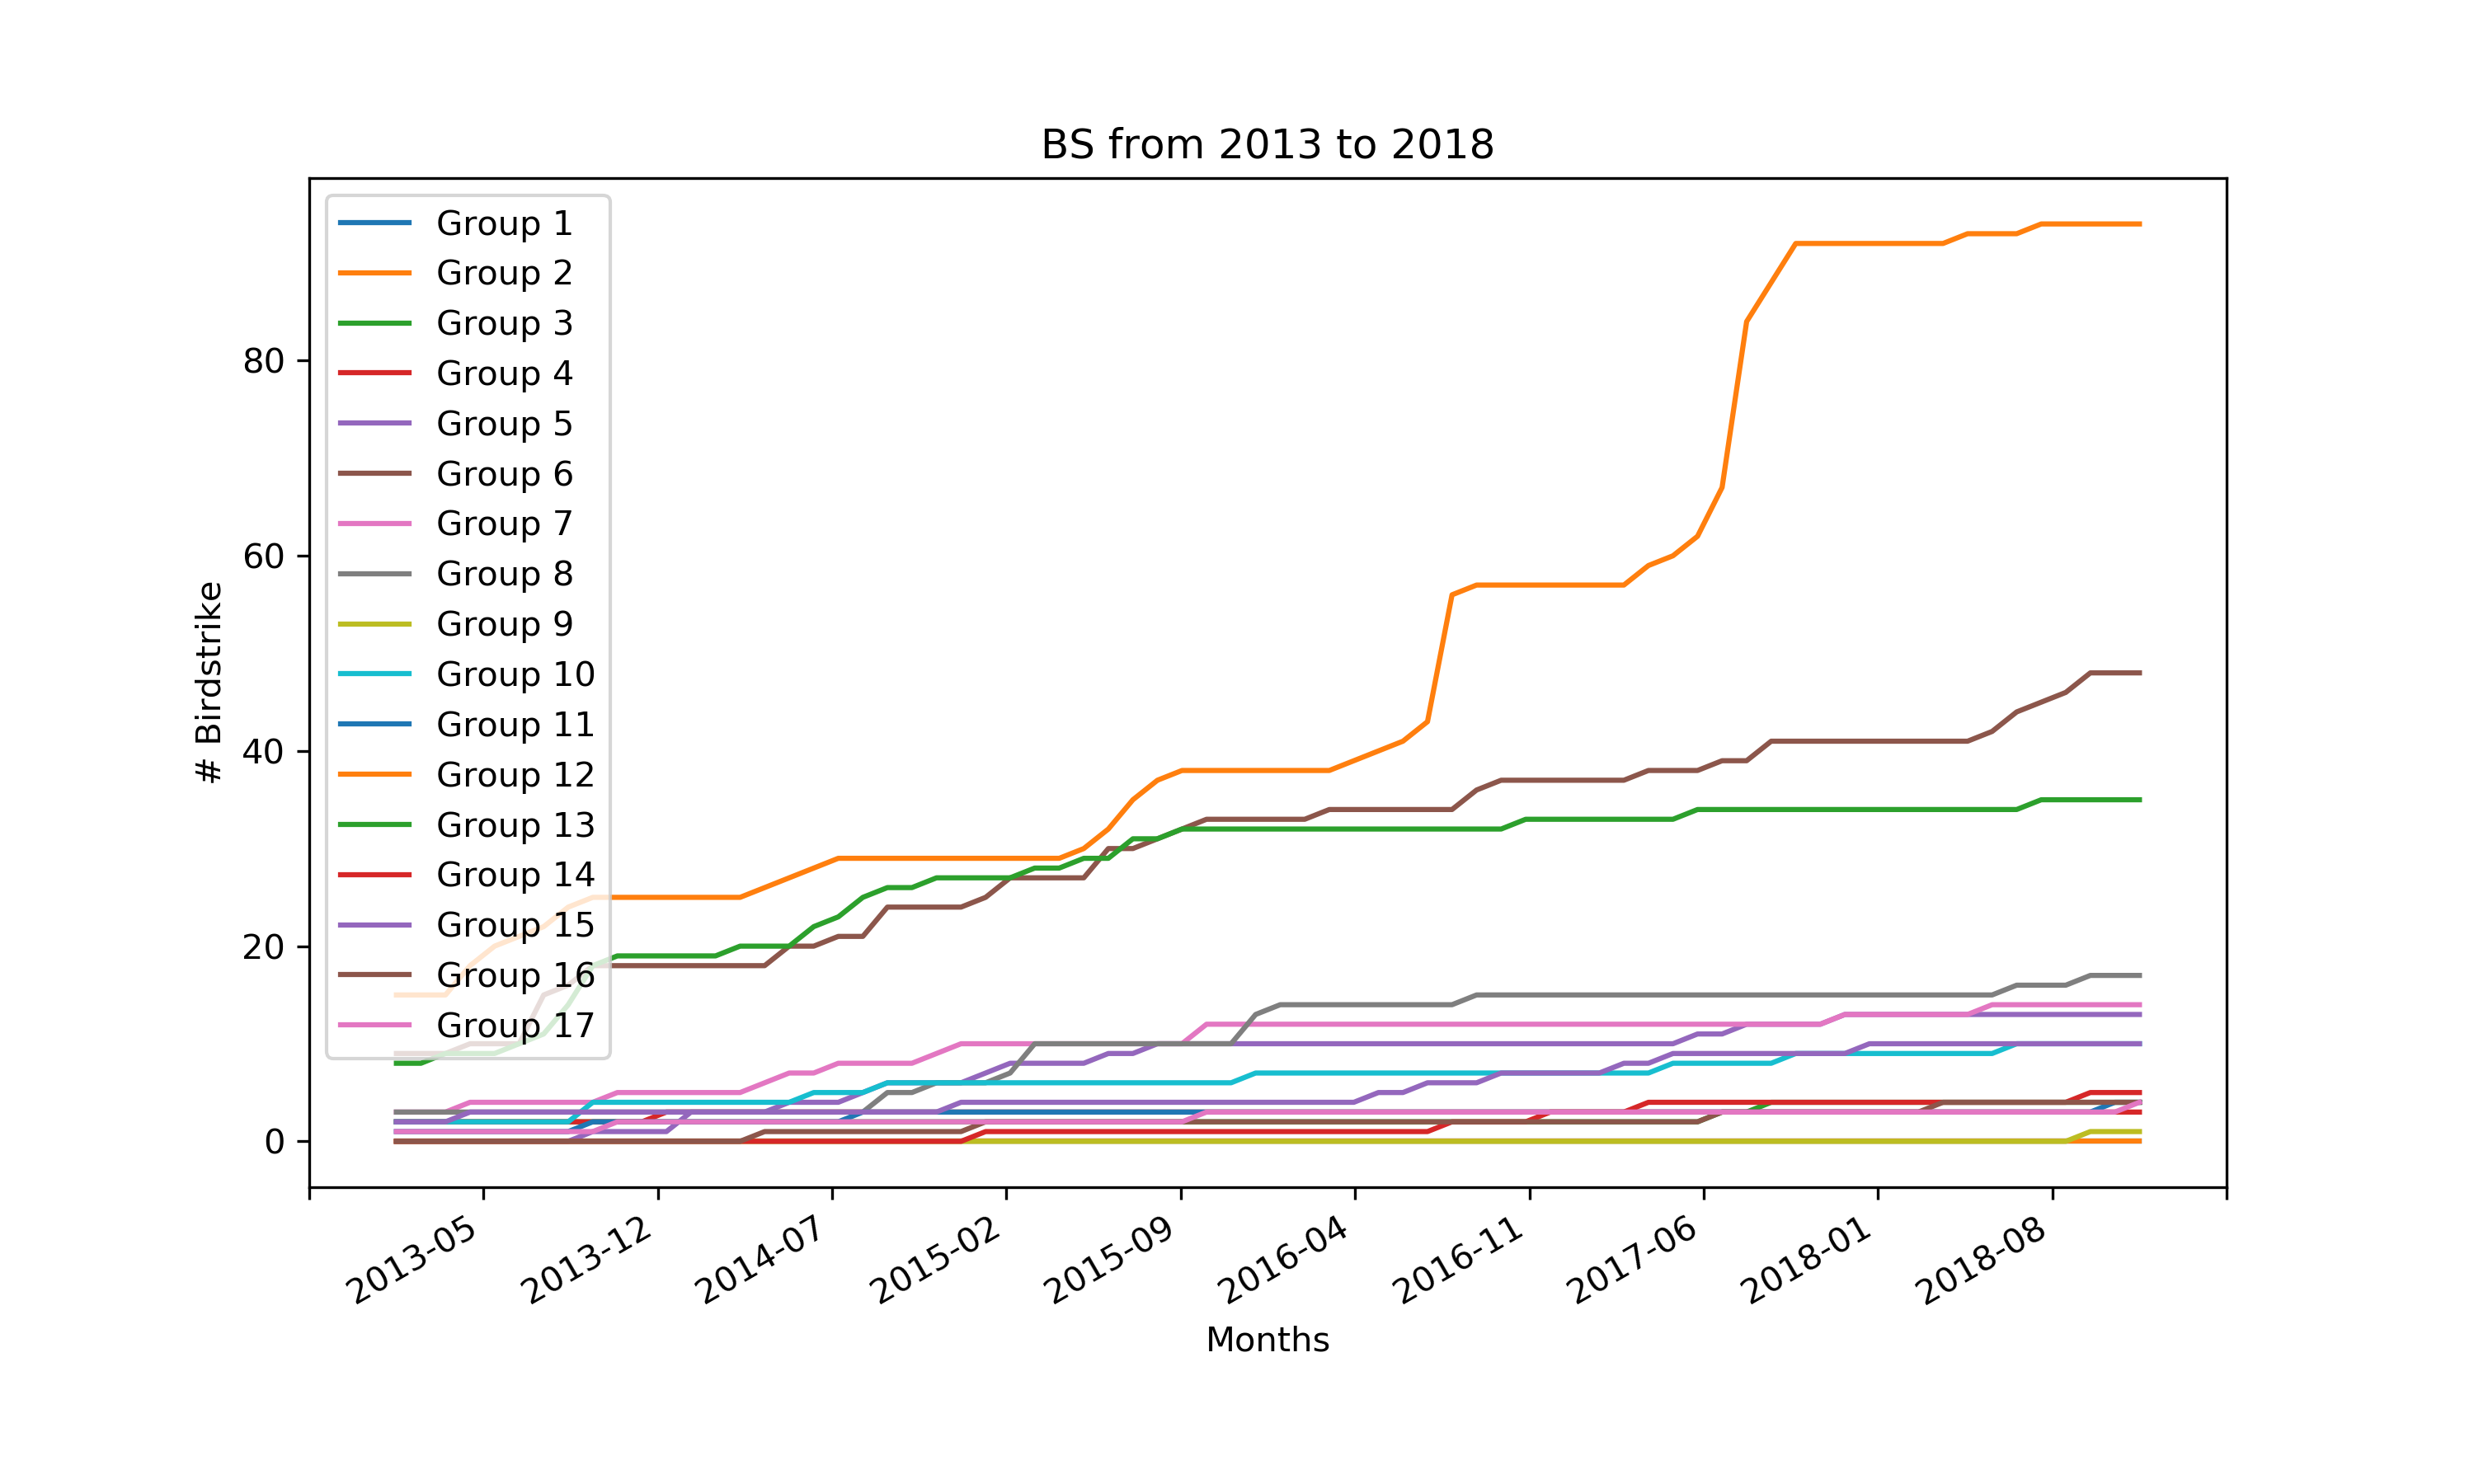
\includegraphics[width=13cm]{img/BS.png}
	\caption{$BS$ parameter from 2013 to 2018 for Pisa airport. The figure shows how, over the years analyzed, the unaveraged $BS$ parameter contributes to a ranking among the species groups.}
	\label{BS_fig}
\end{figure}

The $BS$ parameter is closely related to $EOF^{95}$. This parameter identifies the severity of the birdstrike events for each group and is calculated monthly as the 95th percentile of the $EOF$ values, Table \ref{tab-EOF}. This means that $EOF^{95}$ increases the value of $BS$ and the group factor according to the severity of the birdstrike events, or leaves them unchanged as its minimum value is 1. In Figure \ref{EOF_fig} the $EOF^{95}$ value for each functional group is reported.

\begin{figure}
	\centering
	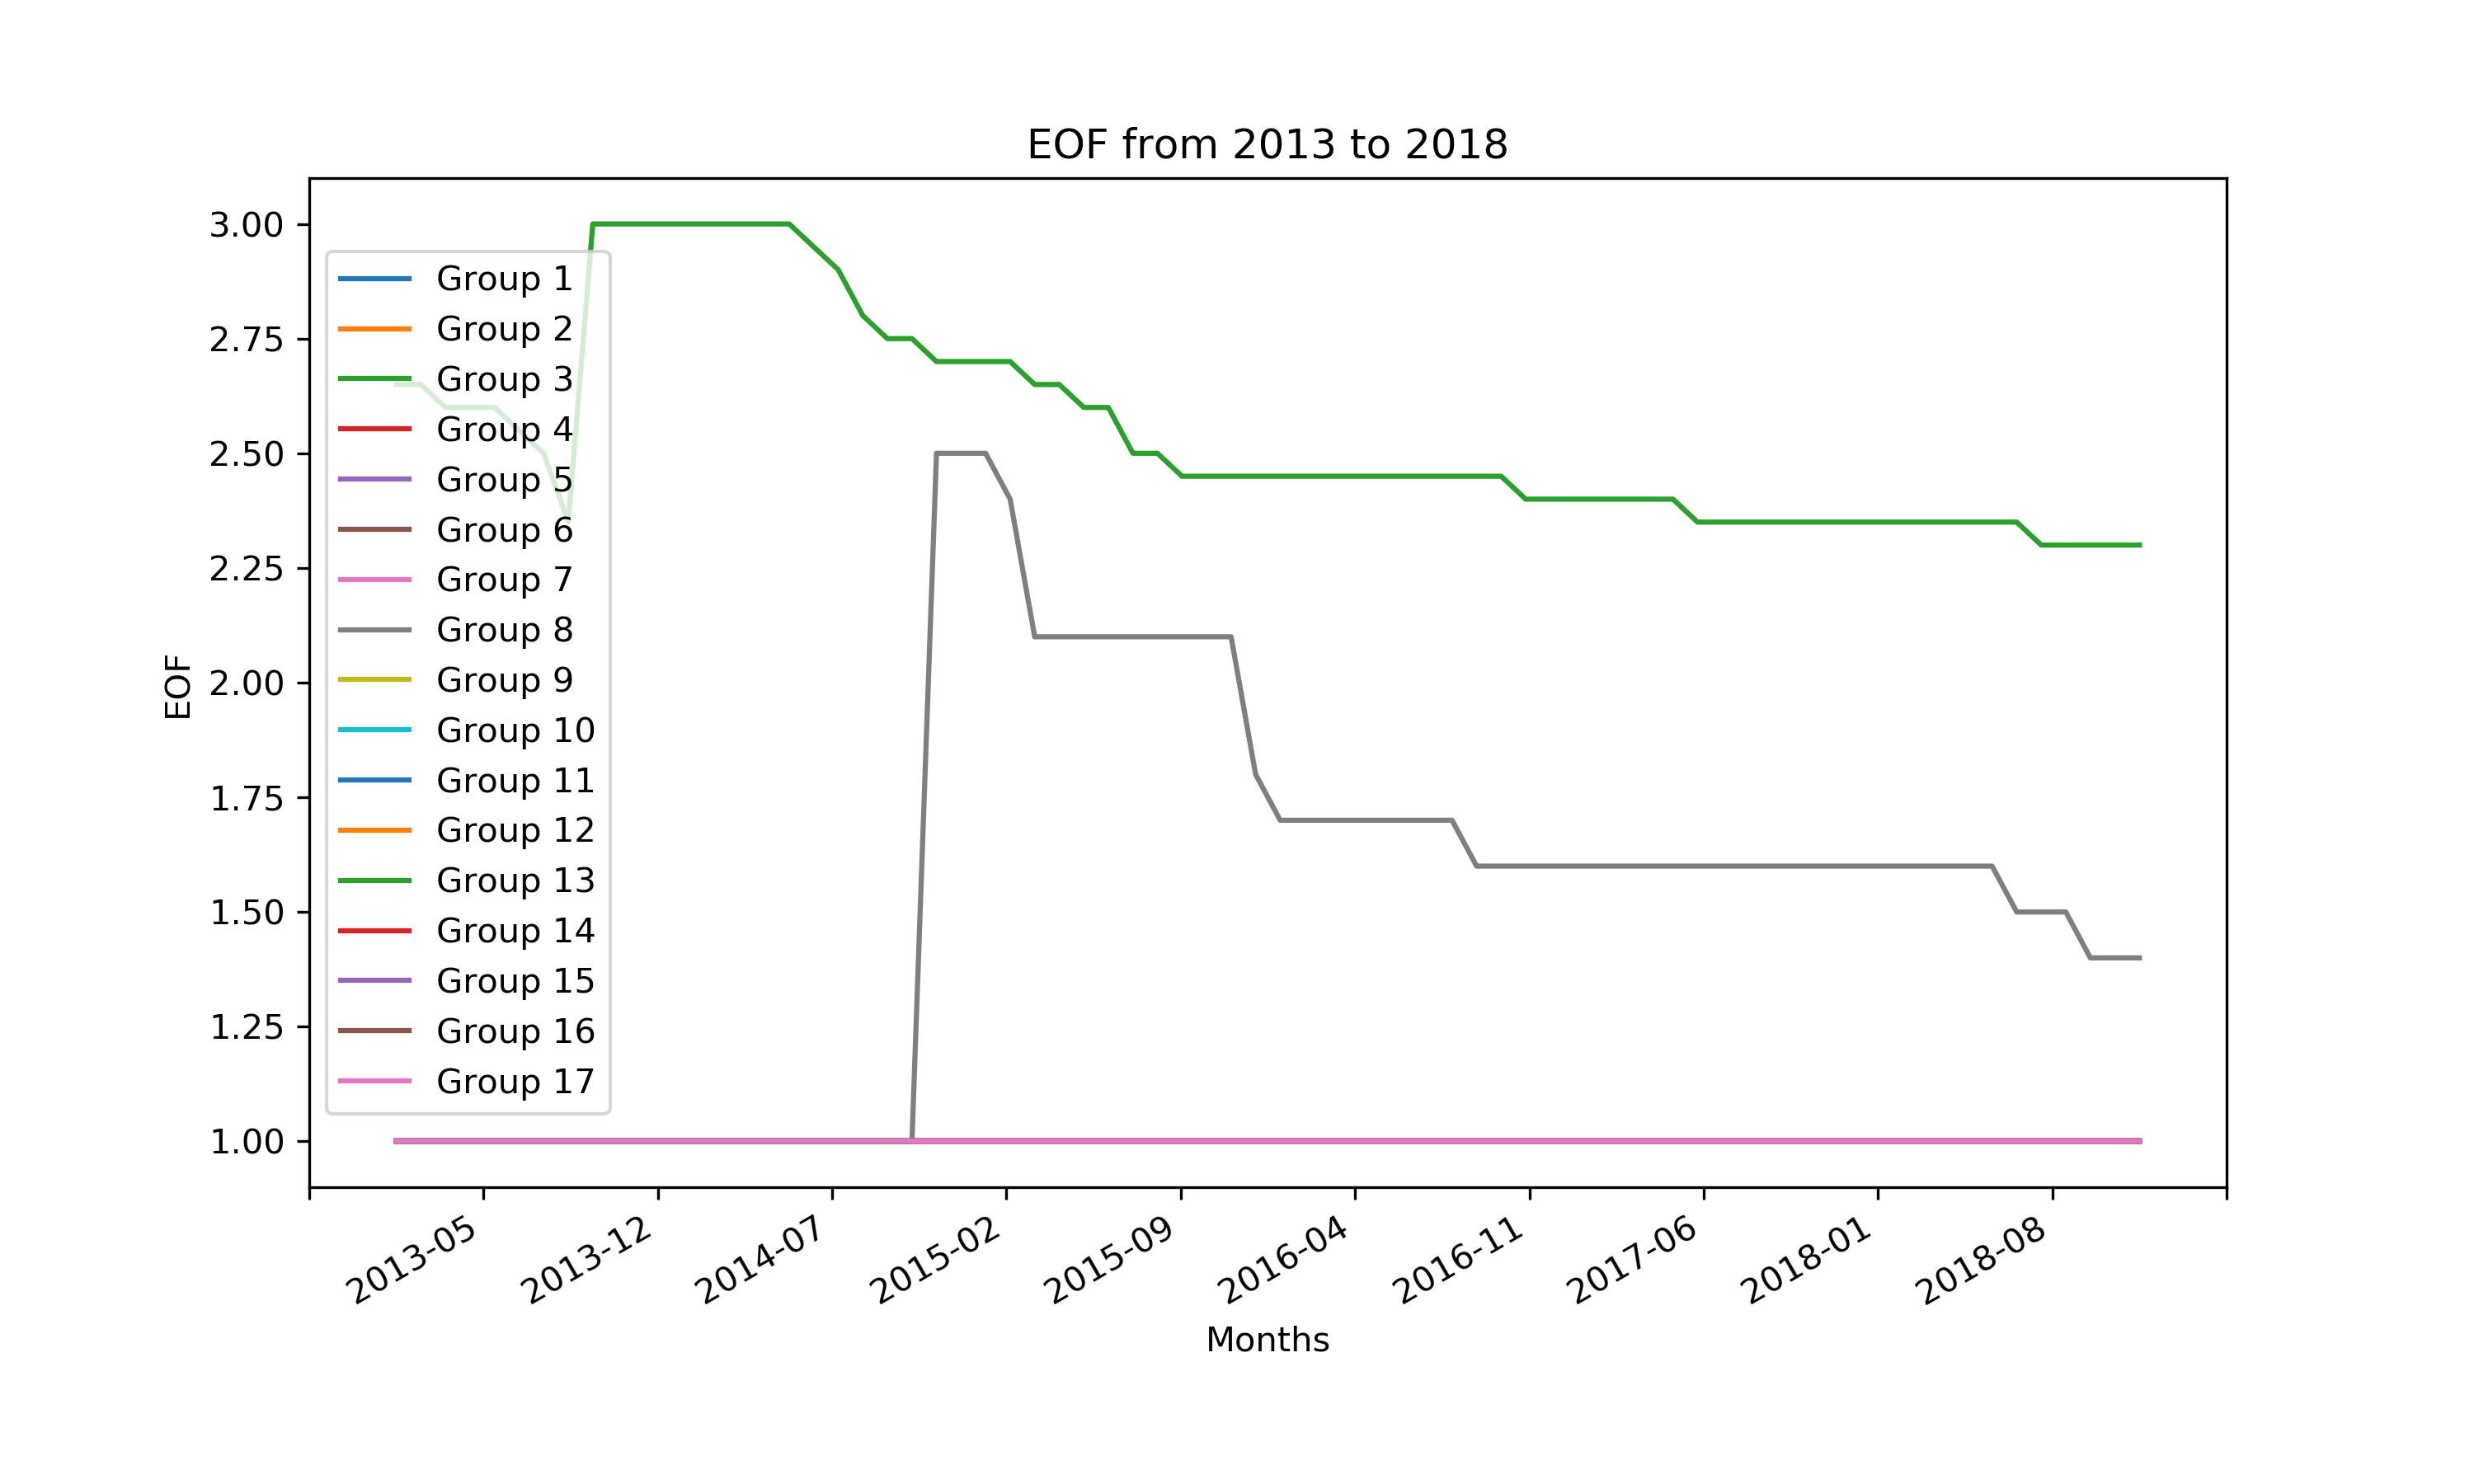
\includegraphics[width=13cm]{img/EOF.png}
	\caption{$EOF^{95}$ parameter from 2013 to 2018 for Pisa airport. The figure shows which group of species has detected birdstrike events with effects on flight. In particular, only 2 groups found these types of events from 2013 to 2018.}
	\label{EOF_fig}
\end{figure}

Another interesting analysis was focused on $Ag$. This parameter is based on sightings and is the average number of flocks sighted at the airport since the monitoring activity started.
The goal of this analysis was to understand the sensitivity of $Ag$ and the contribution of sightings over time as it is averaged on the $BRI_2$ calculation time.
The experiment done was to manually enter sightings in selected months. The months 2014-01 and 2017-12 were chosen to emphasize the desired behavior. In particular, 100 sightings per day were entered for all two months.
The result of the experiment can be seen in Figure \ref{AG_fig}, where the addition of sightings in 2017-02 has a smaller contribution than in 2014-01. This is due to the average over the entire calculation time of the $BRI_2$ and makes the $Ag$ parameter less sensitive to sightings.
\begin{figure}
	\centering
	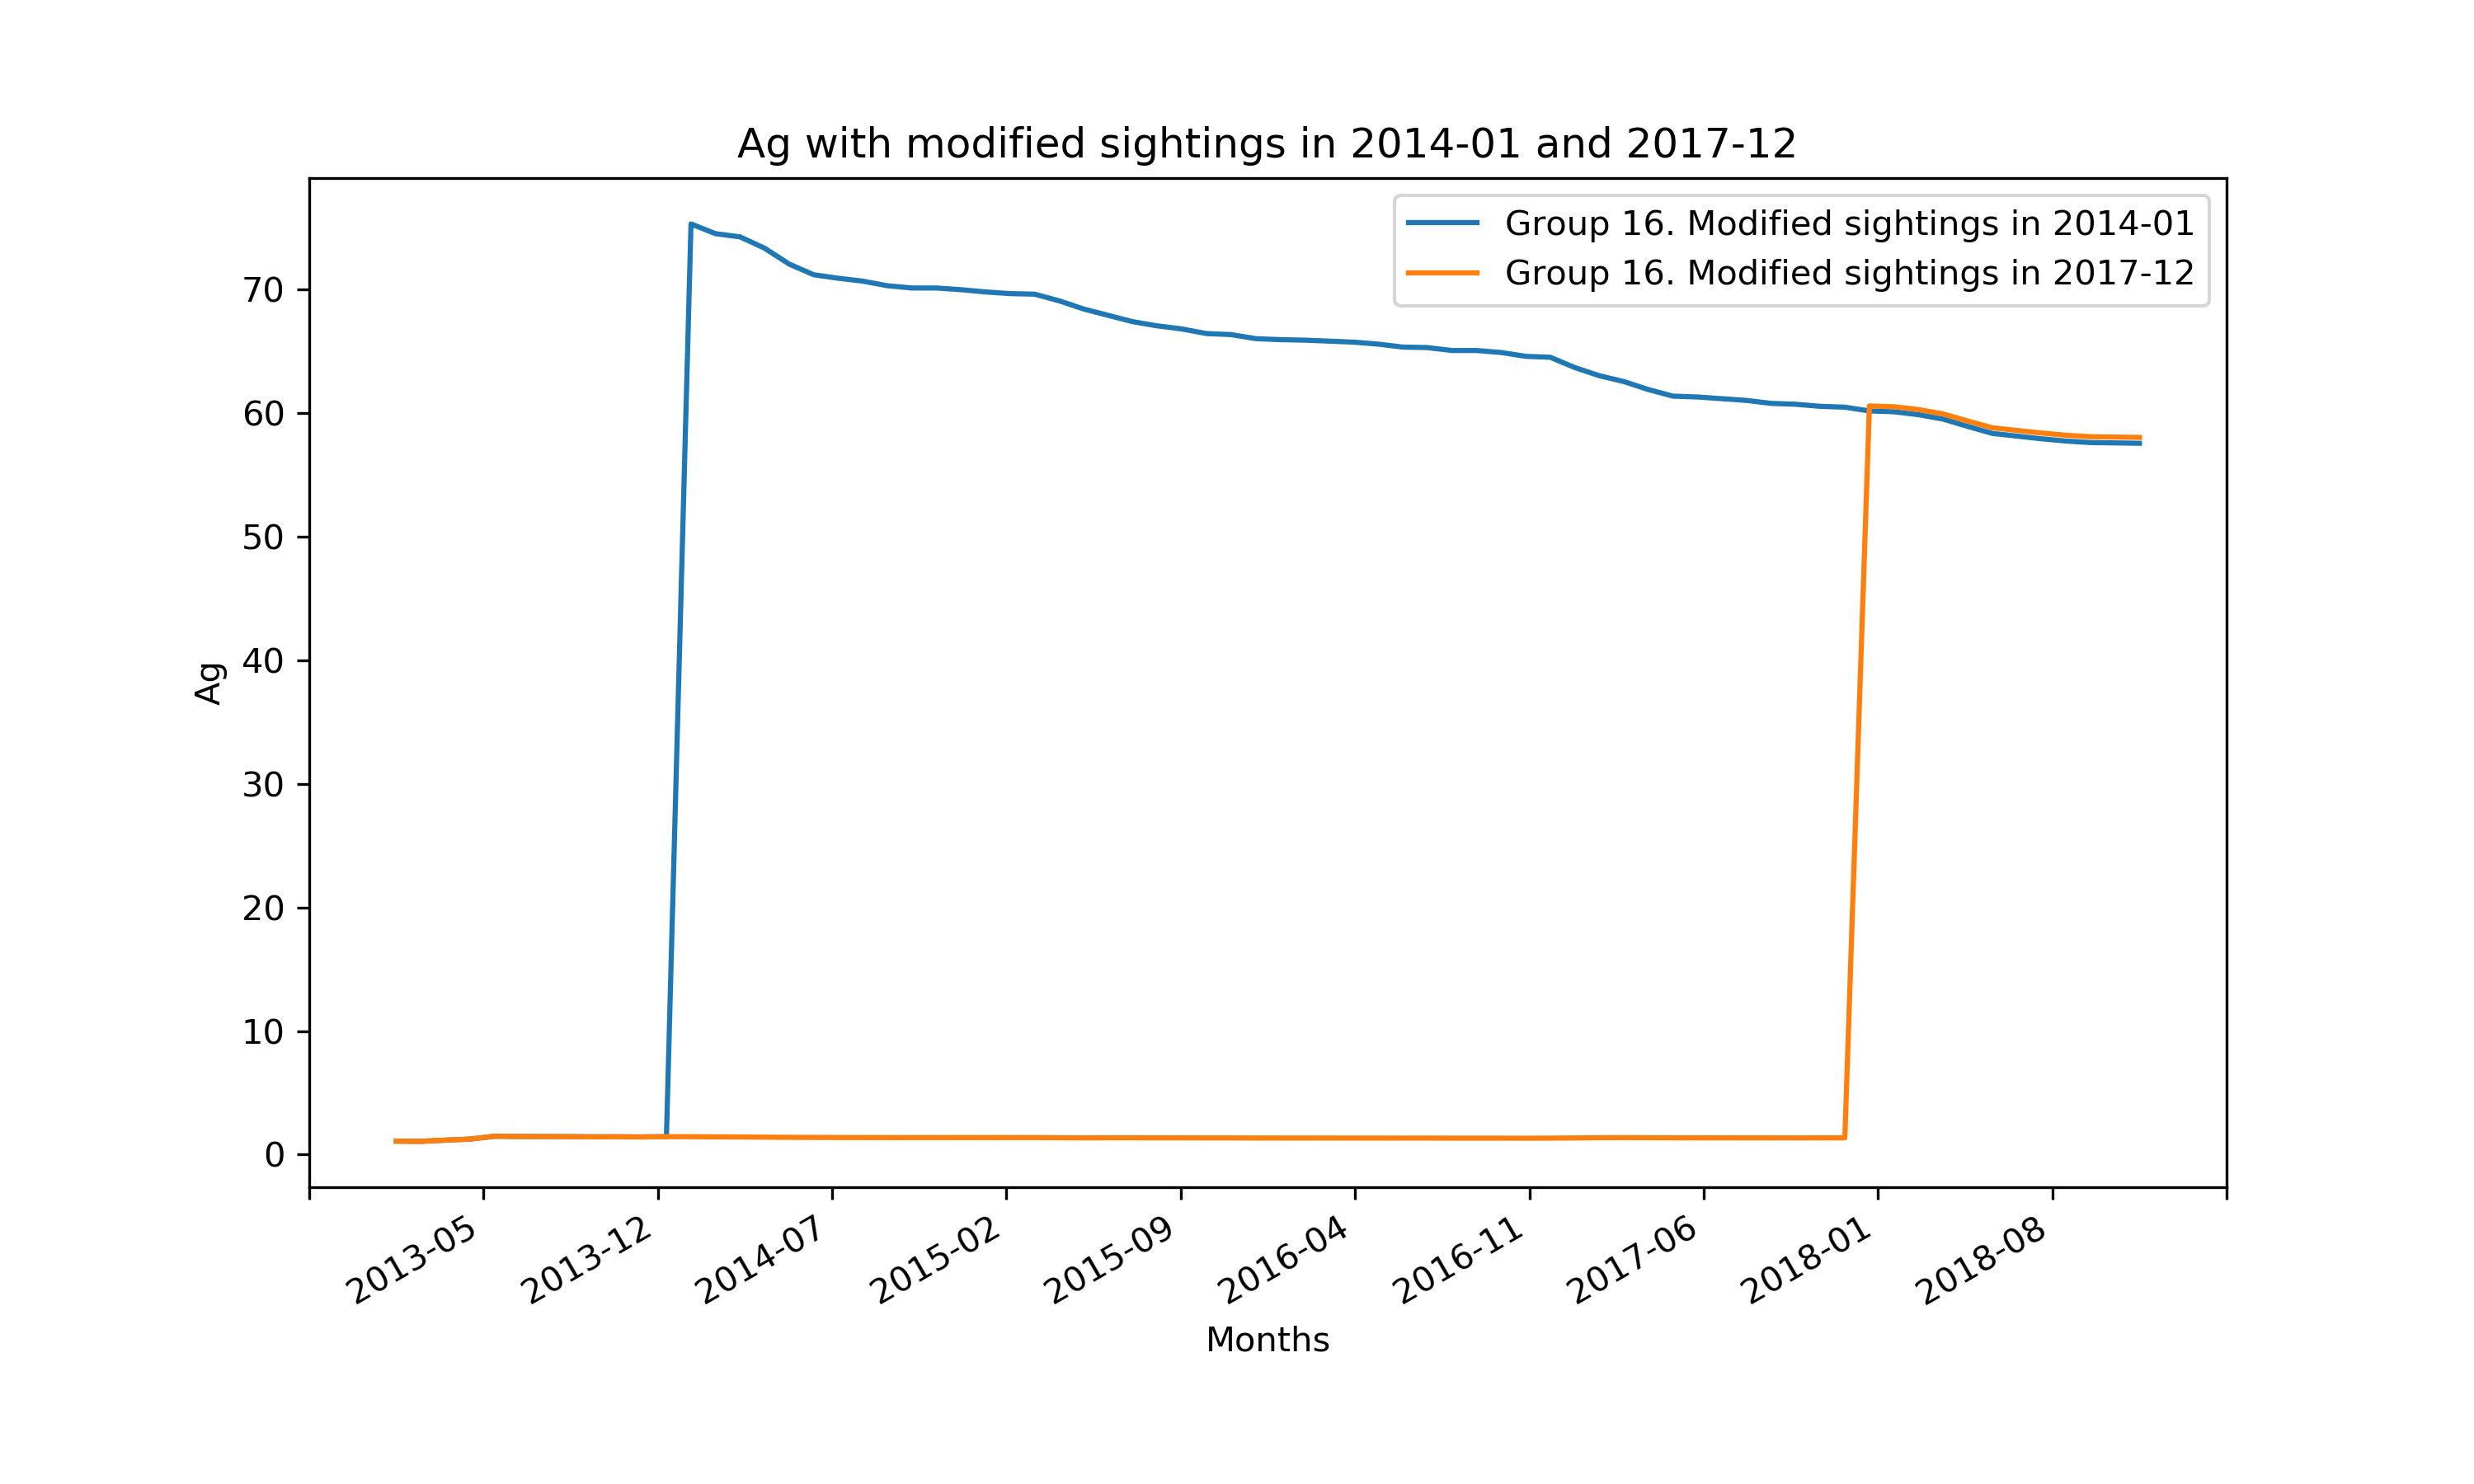
\includegraphics[width=13cm]{img/AG.png}
	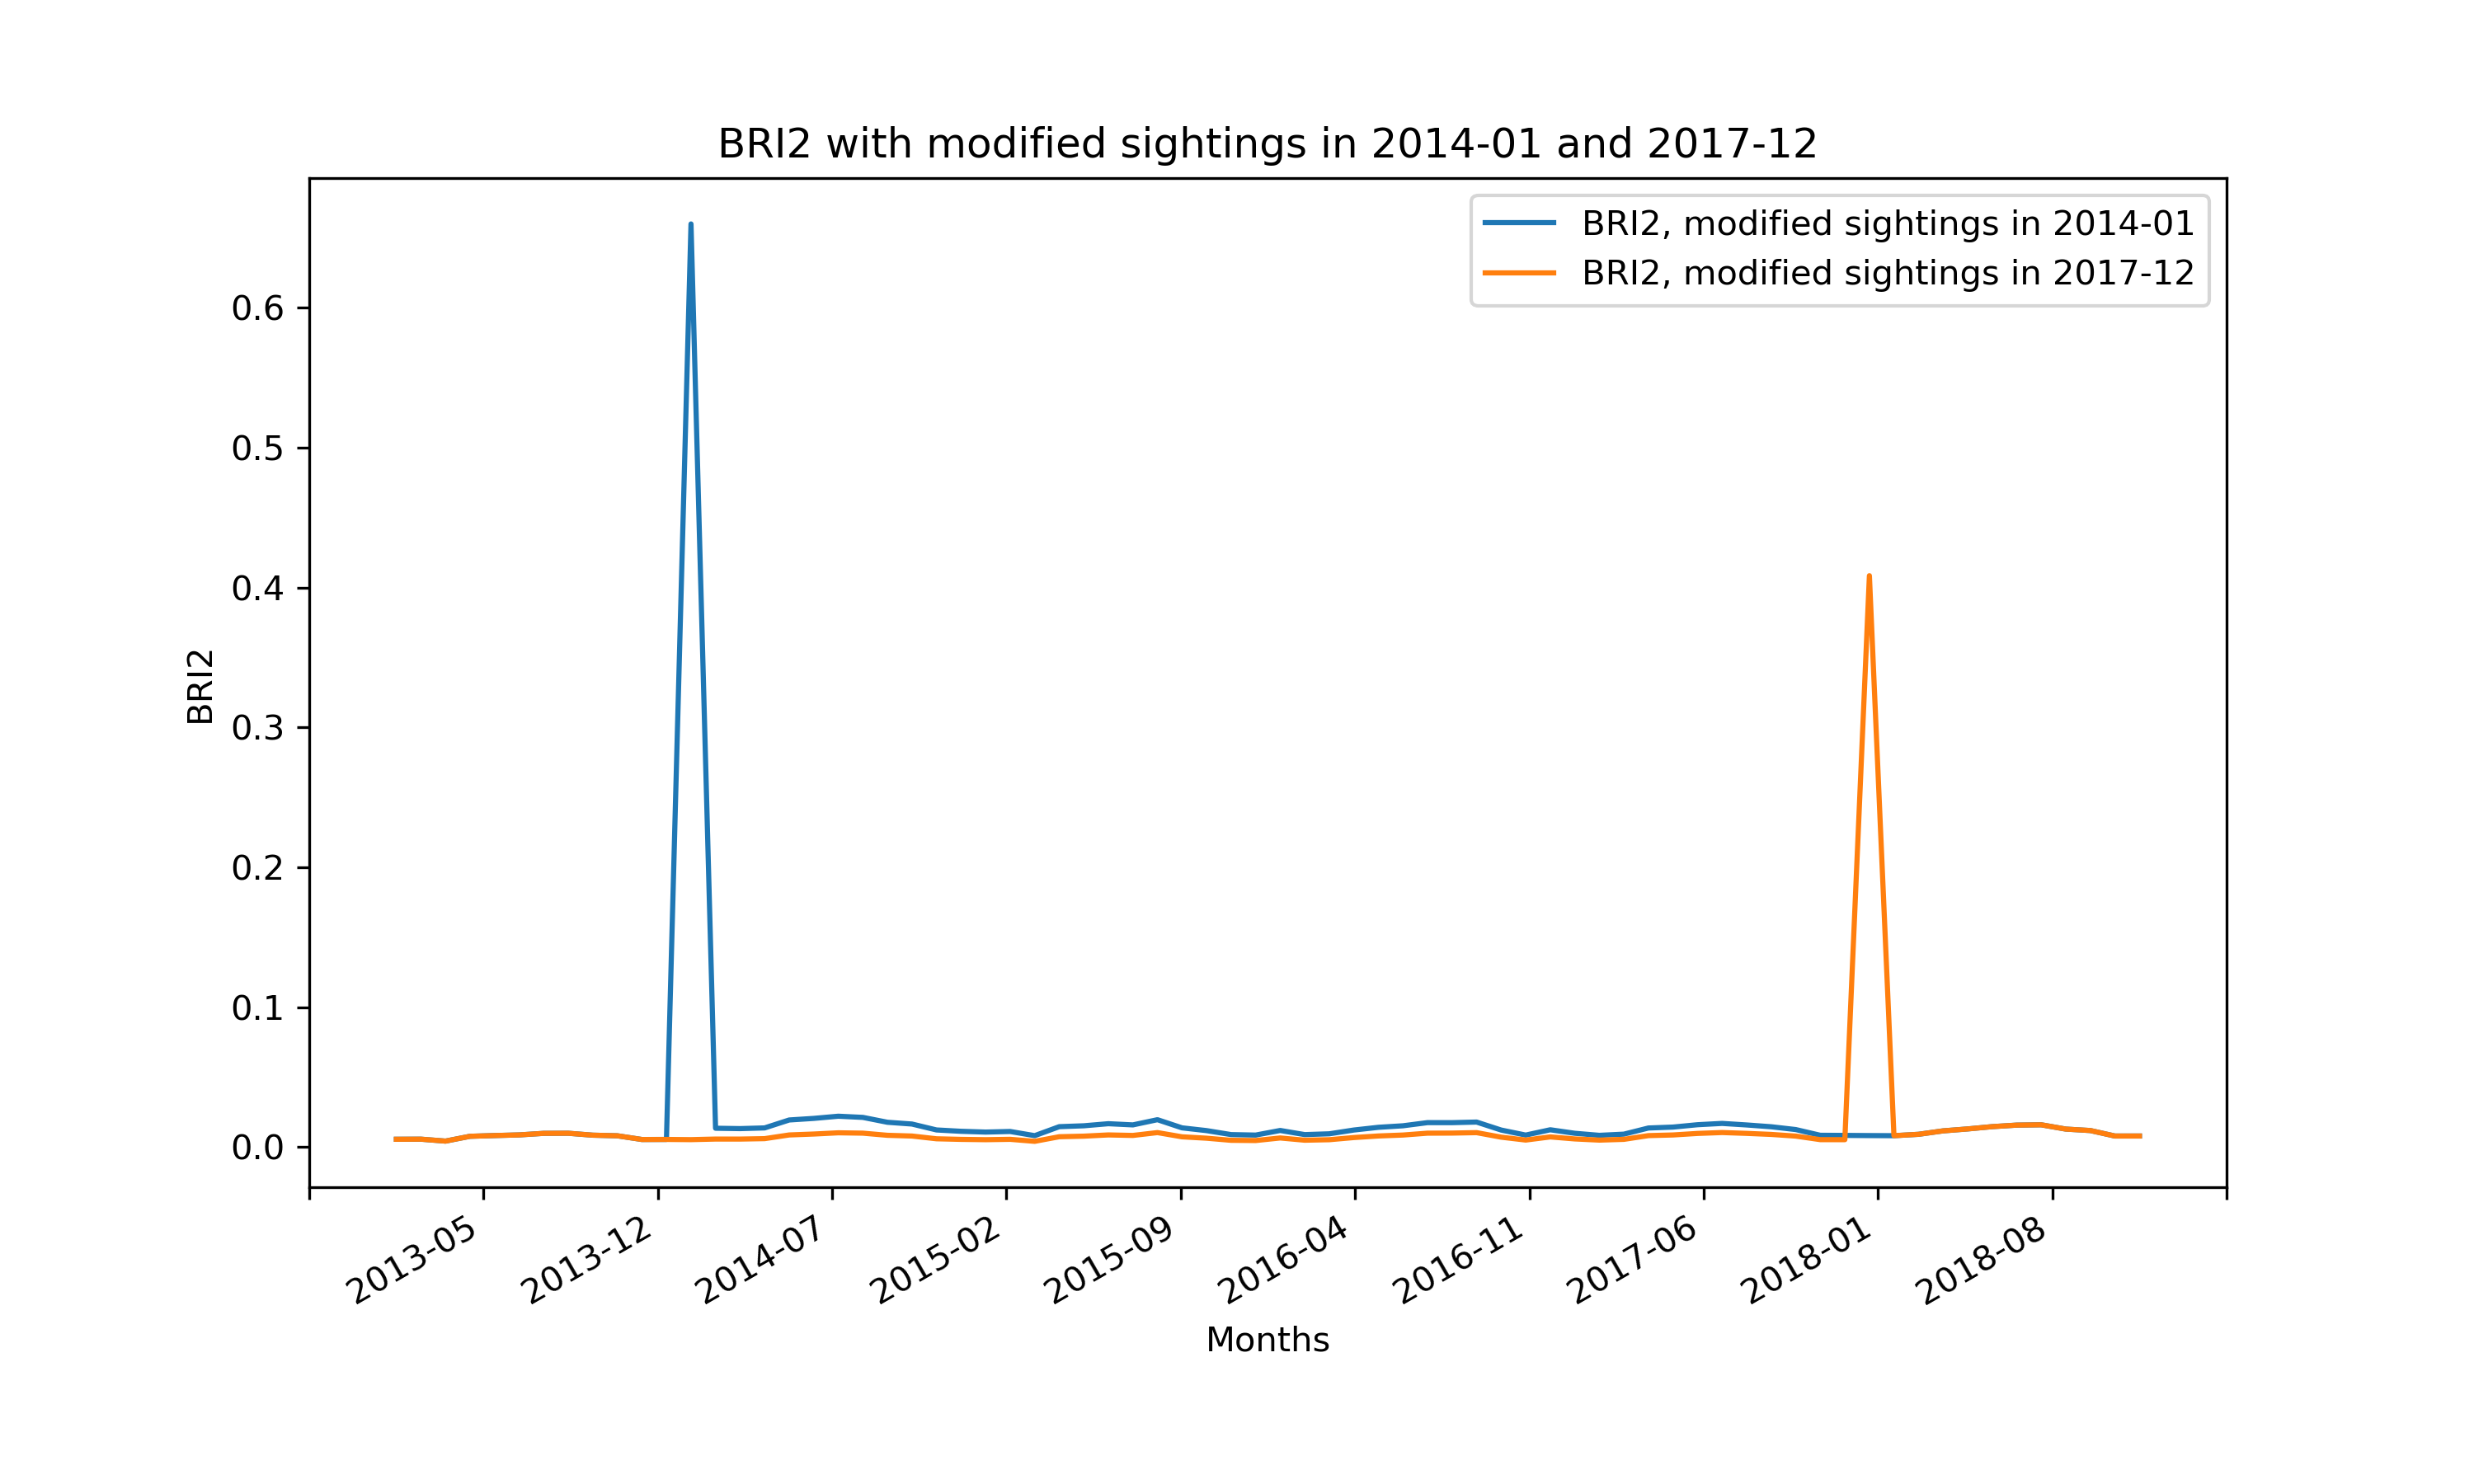
\includegraphics[width=13cm]{img/BRI2_c.png}
	\caption{$Ag$ and $BRI_2$ parameter with modified sightings in 2014-01 and 2017-12. The figure shows (above) the effect of the average on the $Ag$ parameter. This causes the effect of sightings to degrade over time. In particular it has been shown the effect on 1 group out of 17. The figure (below), shows the effect of the average $Ag$ in the $BRI_2$ calculation. This causes a degradation of the effect of sightings over time that is also observed in the $BRI_2$ value.}
	\label{AG_fig}
\end{figure}
This behaviour can also be observed in the calculation of the $BRI_2$ by making the group factor depend exclusively on sightings. The rusult of this experiment is shown in Figure \ref{AG_fig}.
No specific analysis has been made for the remaining parameters. In particular $TFN$ and $\overline{TFN}$ are normalizers for equations \ref{eq:3.2} and \ref{eq:3.3} and $DB$ is a daily average of sightings  not dependent on time.

After these analyses it is clear that the fundamental parameters for the calculation of $BRI_2$ are $BS$, $Ag$, $EOF^{95}$. Some problems have been identified:
\begin{itemize}
    \item $Ag$ loses sensitivity to sightings over time.
    \item  $BS$ is a cumulative parameter that stores birdstrike events from the beginning of the $BRI_2$ calculation and is not averaged.
    \item  $EOF^{95}$ contributes to the group factor increase by boosting the effects of $BS$.
\end{itemize}
The group factor $GF$ can be considered as a sort of reputation among the species groups that over time creates a ranking of danger gradually less related to sightings but closely related to the birdstrike events of the past.
This means that the $BRI_2$ value will be higher if more dangerous groups are sighted independently to the amount of elements sighted.

\section{Correlation with wildlife strike events}\label{smooth}
A second study has been done to understand if $BRI_2$ is a good
tool capable of describing an airport-specific wildlife strike risk.
If $BRI_2$ is a good risk-index it must have a good correlation with the events of wildlife strike.

The first step of this study was to generate a curve that would describe as accurately as possible the evolution of wildlife strike events over time.
To generate the curve a Gaussian filter was chosen and correlation tests were performed with different $\sigma$ values (standard deviation for Gaussian kernel), in particular $\sigma = [0.5, 1.0, 1.5, 2.0]$, and for comparison $BRI_2$ and the curve of wildlife events have been normalized.

The measure of correlation chosen was the correlation of Spearman. It estimates how well the relationship between two variables can be described using a monotonous function. The sign of the Spearman correlation indicates the direction of association between $X$ (the independent variable) and $Y$ (the dependent variable). If $Y$ tends to increase when $X$ increases, the Spearman correlation coefficient is positive. If $Y$ tends to decrease when $X$ increases, the Spearman correlation coefficient is negative. A Spearman correlation of zero indicates that there is no tendency for $Y$ to either increase or decrease when $X$ increases.
Equation \ref{eq_spearman} show the formula for the calculation of the Spearman correlation for a sample of size n. The n raw scores $X_i, Y_i$ are converted to ranks rg($X_i$), rg($Y_i$) and $\mathit{r_s}$ is computed as:

\begin{equation}\label{eq_spearman}
\mathit{r_s} = \frac{\mathrm{cov(\mathrm{rg_\mathcal{X}}, \mathrm{rg_\mathcal{Y}}})}{\sigma_{\mathrm{rg_\mathcal{X}}}\sigma_{\mathrm{rg_\mathcal{Y}}}}
\end{equation}
where:

\begin{itemize}
    \item $\mathrm{cov(\mathrm{rg_\mathcal{X}},\mathrm{rg_\mathcal{Y}}})$ is the covariance of the rank variables.
    \item $\sigma_{\mathrm{rg_\mathcal{X}}}\sigma_{\mathrm{rg_\mathcal{Y}}}$ are the standard deviations of the rank variables.
\end{itemize}
Only if all n ranks are distinct integers, it can be computed using the formula in equation \ref{eq_spearman_2}:

\begin{equation}\label{eq_spearman_2}
\mathit{r_s} = 1 - \frac{\sum_{i} d^2_i}{n-(n^2-1)}
\end{equation}
where $d_i$ = rg($X_i$), rg($Y_i$).

It is possible to observe the result of the study for Pisa airport in Figure \ref{corr_curve} and \ref{corr_scatter}.
\begin{figure}
	\centering
	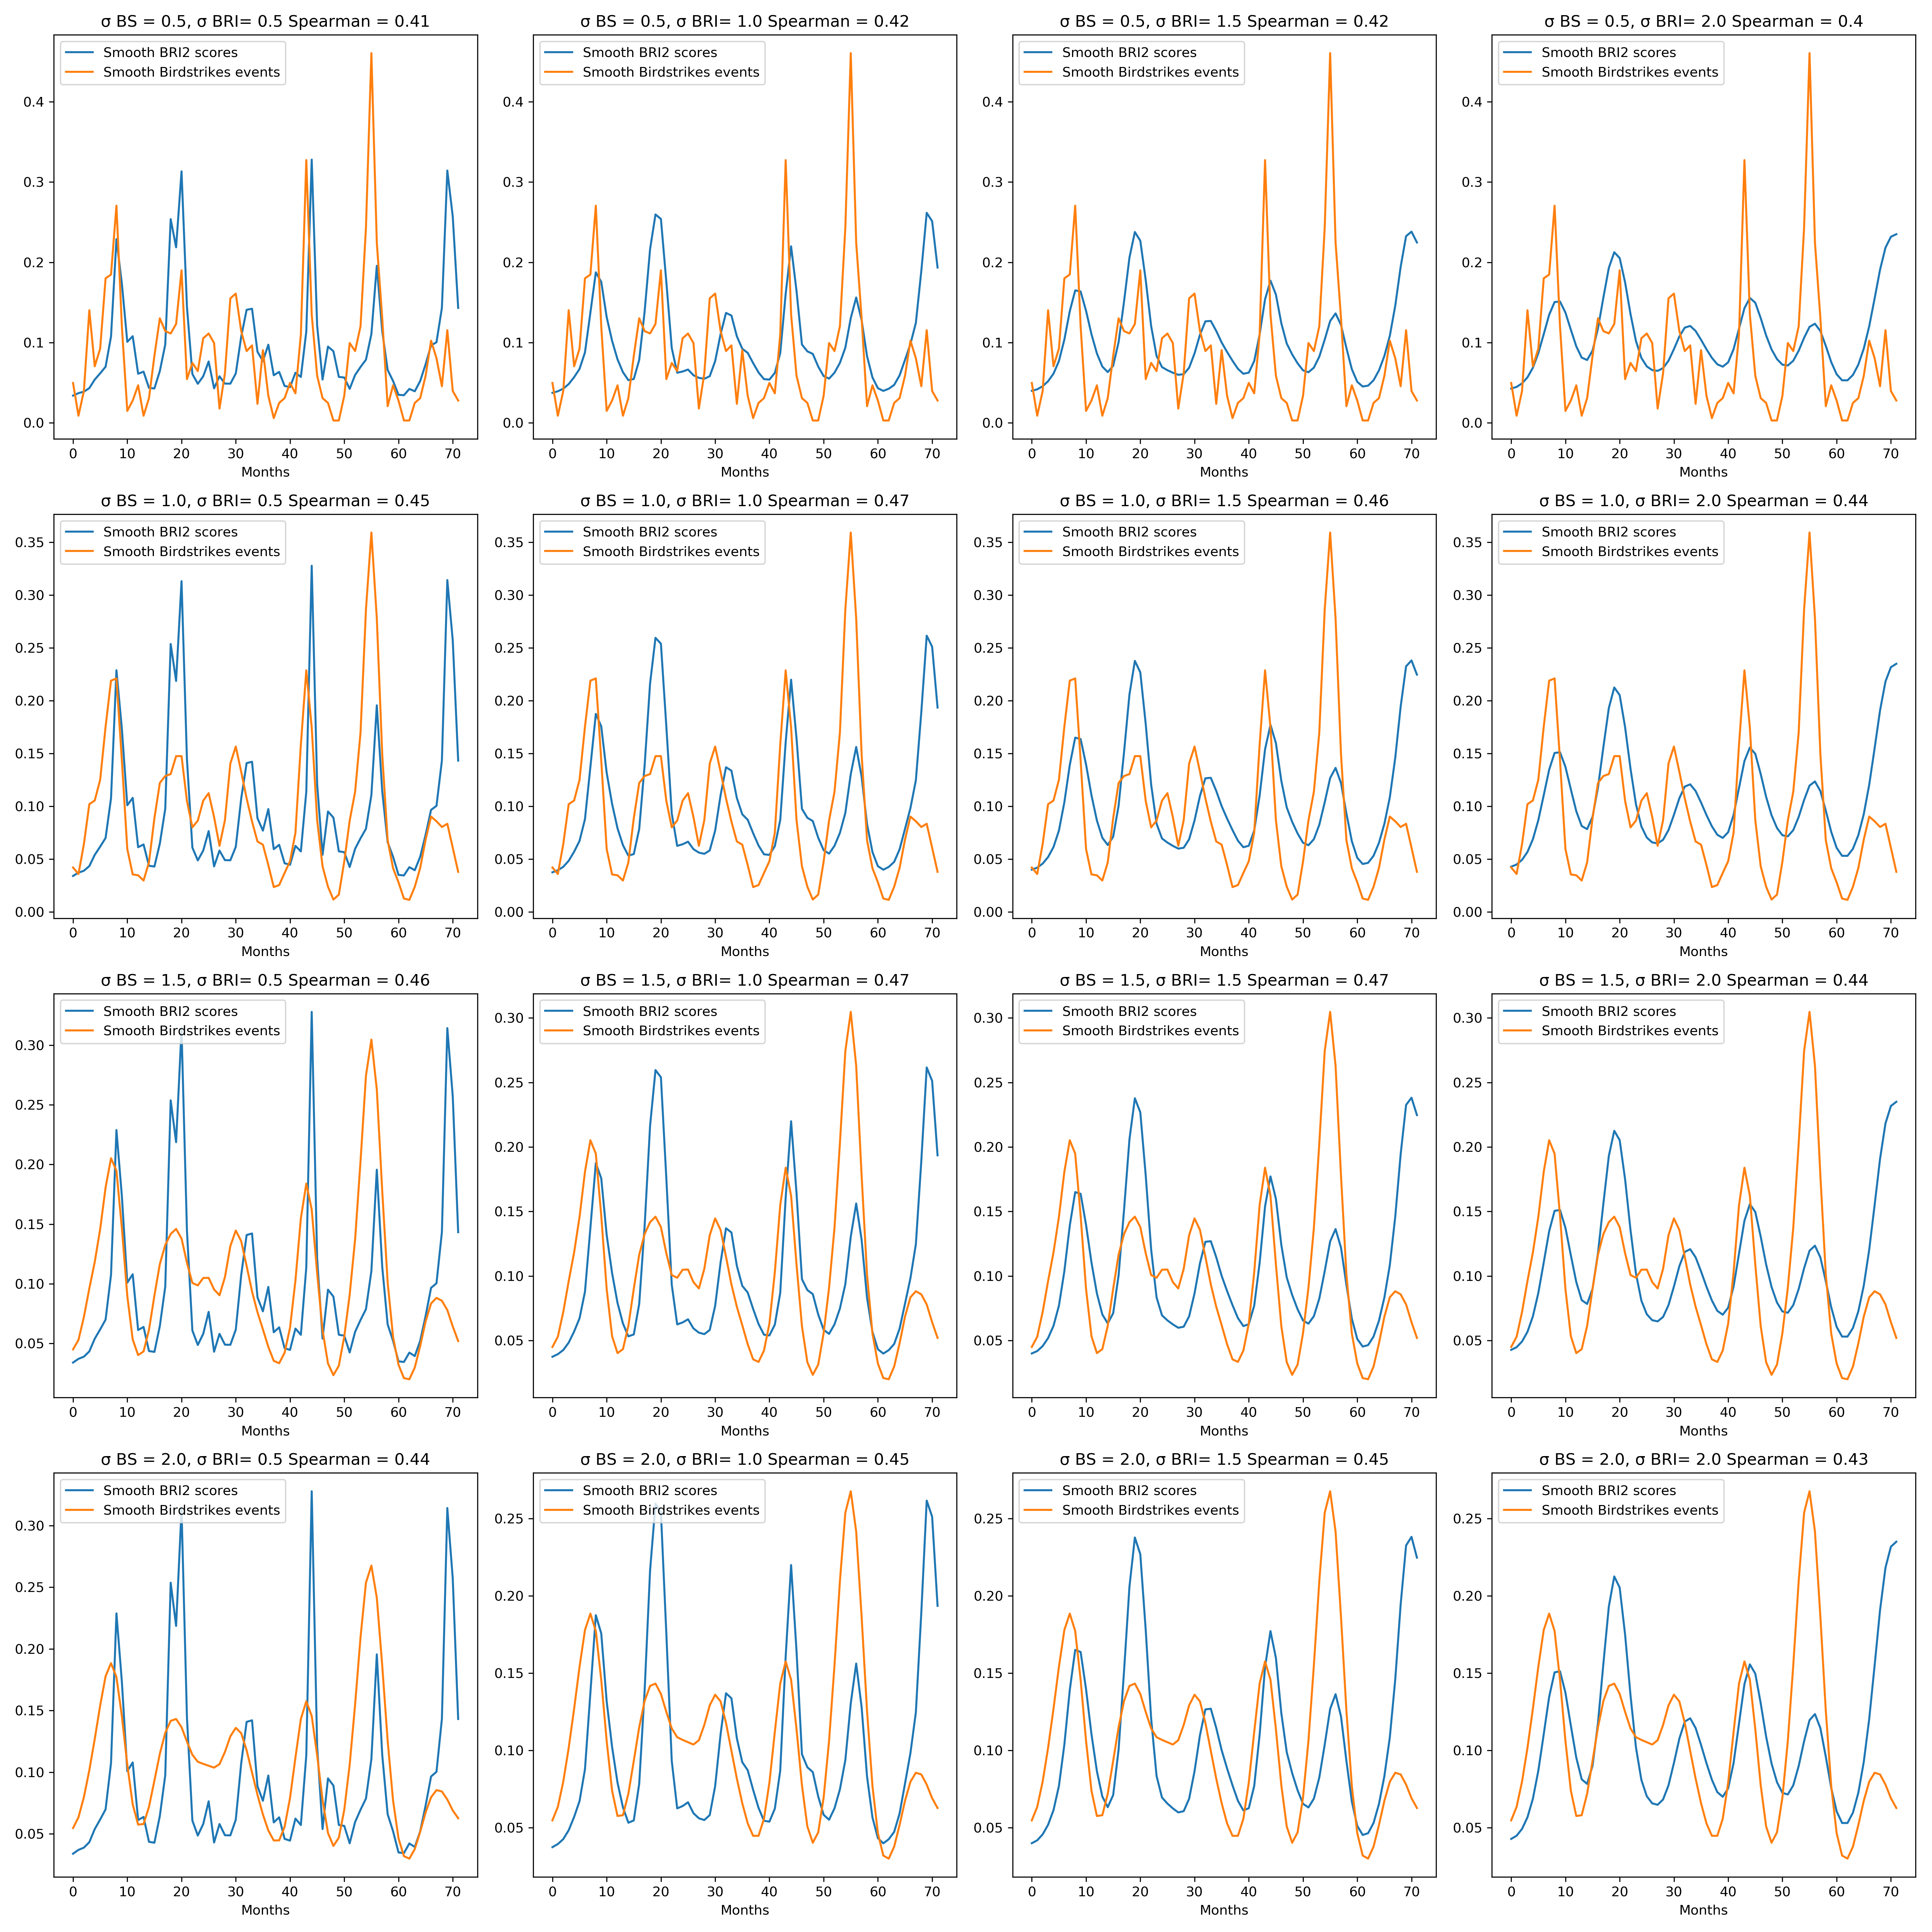
\includegraphics[width=14cm]{img/corr_curve.png}
	\caption{Spearman correlation between $BRI_2$ and the wildlife strike curve. Each subplot shows the correlation between the two variables with a different level of smoothing given by the Gaussian filter.}
	\label{corr_curve}
\end{figure}
\begin{figure}
	\centering
	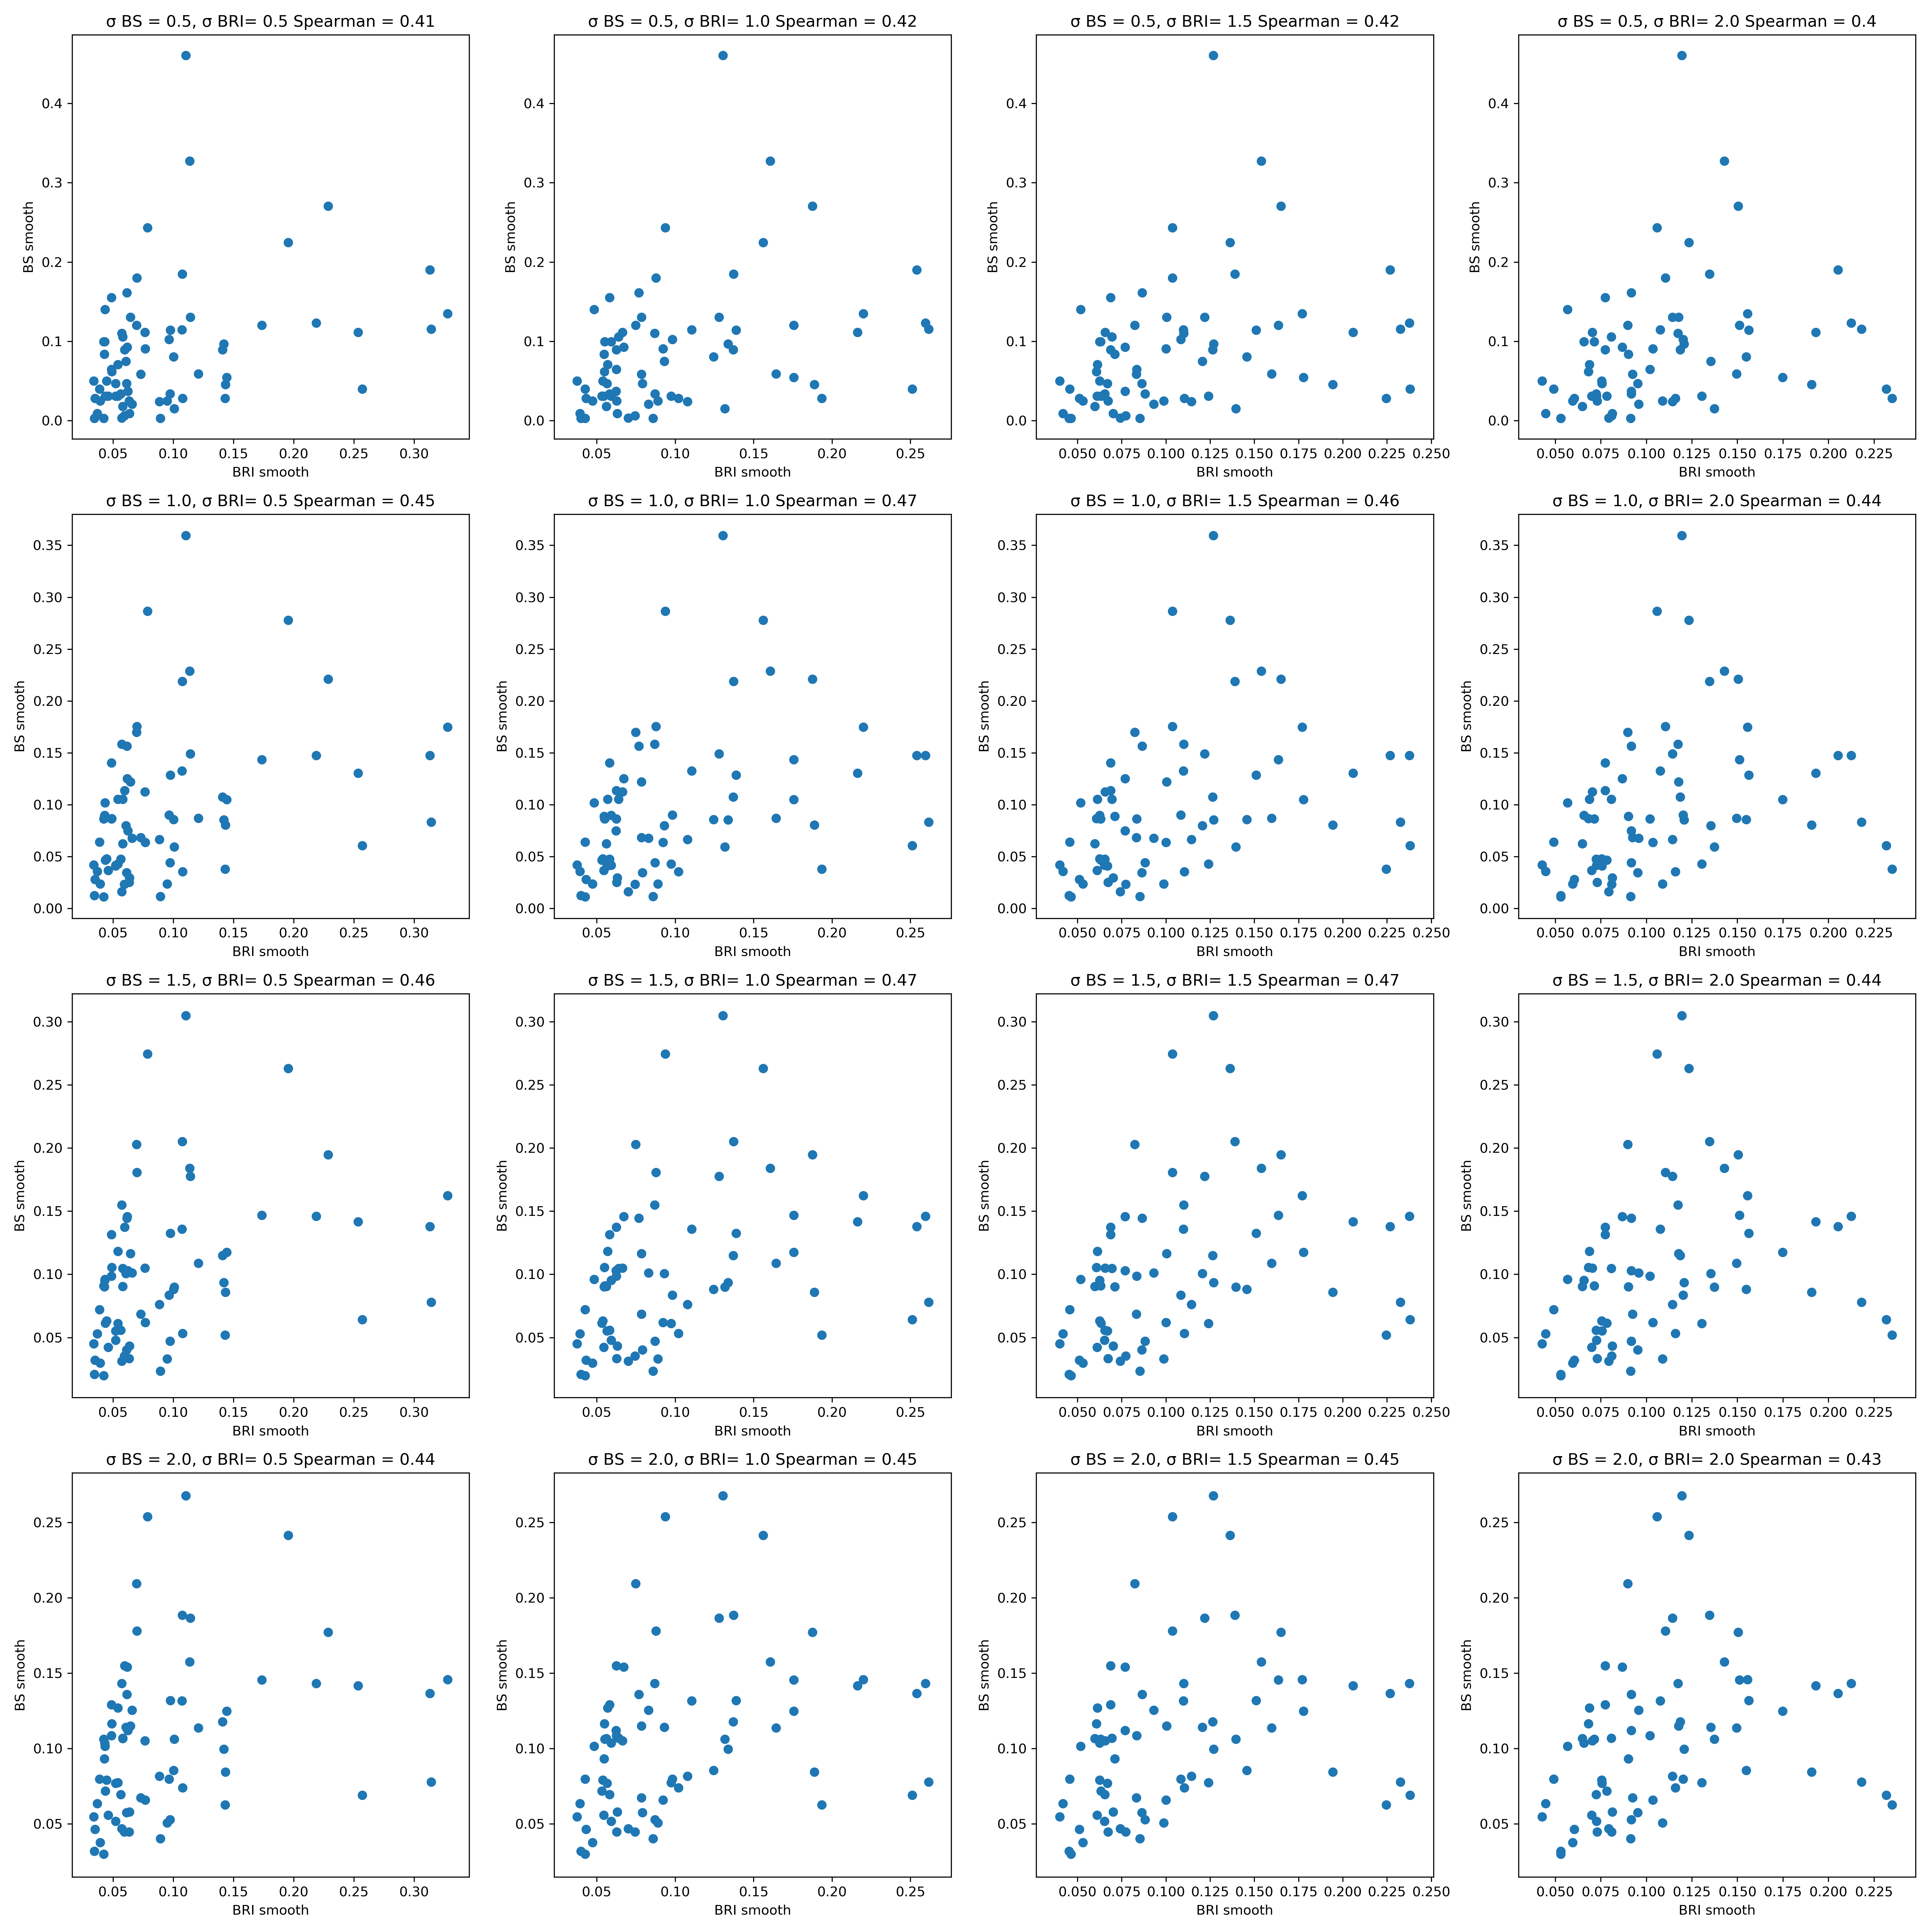
\includegraphics[width=14cm]{img/corr_scatter.png}
	\caption{Spearman correlation between $BRI_2$ and the wildlife strike curve. Each scatter-subplot shows the correlation between the two variables with a different level of smoothing given by the Gaussian filter.}
	\label{corr_scatter}
\end{figure}
Each subplot shows the Spearman correlation between the two variables with a different level of smoothing given by the Gaussian filter.
In particular, in Figure \ref{corr_scatter} scatter plots are used to display $BRI_2$ and wildlife strikes' values in cartesian coordinates.
The results show that for Pisa at most Spearman correlation has value 0.47, obtained in 3 cases out of 16, which means a not so high correlation.

\begin{table}
	\centering
	\scalebox{1}{
	\begin{tabular}{@{}ccc@{}}
		\toprule
		Airport & Spearman correlation \\	\midrule
		Florence & 0.17 \\
		Pisa & 0.47 \\
		Bologna & 0.26\\
		Milan-Malpensa &  -0.14 \\
		Milan-Linate & -0.28 \\
		Verona & 0.6 \\
		Catania & 0.49 \\
	    Brescia & 0.31 \\	\bottomrule
	\end{tabular}}
	\caption{Correlation values between $BRI_2$ and wildlife strikes events of some Italian airports.}
	\label{tab-corr}
\end{table}

The Table \ref{tab-corr} shows the results of the correlation in other Italian airports. Also for other airports the correlation with wildlife events is not so high, where the highest correlation found was 0.5 at Catania airport.

The next chapter deals with the proposed model. The purpose of this model is to provide a new risk-index closer related to $BRI_2$.

\subsection{Discussion}

After the analysis performed and discussed in this chapter, the $BRI_2$ risk index is dependent on variables (described in \ref{Formula_explanation}) which are certainly easy to explain and understand. But this makes the $BRI_2$ an easy to calculate but empirical index.
We have identified in section \ref{parameters_analysis} important problems related to the factors involved:
$Ag$ is a averaged parameter that loses sensitivity over time, $GF$ is a reputation of species groups not very dependent on sightings but related to the number of birdstrike events caused in the past, given the nature of variables $Ag$ and $BS$ which is cumulative over time.
Finally, the $BRI_2$ has proven to be poorly correlated to historical birdstrike events collected on all the airports tested in the analysis (Table \ref{tab-corr}).
